% тут общее описание 2D-МОЛ


\startp
\upar{Поток загрузки}
В соответствии с формулами \eqref{oven}, \eqref{vcrit}, а также считая, что захватываются все атомы со скоростью $v < \vcap$ \cite{hf}
\begin{equation}
	\sub{\Phi}{2d} \propto \sub{\Phi}{tot} \int_{0}^{\vcap} v^3 e^{-v^2/\alpha^2} \d v,
	\hspace{5 mm} 
	\Phi_0 = \sub{n}{sat} \bar{v} \sub{S}{oven} \frac{\sub{\Omega}{2d}}{4 \pi},
	\hspace{0.5cm} \Rightarrow \hspace{0.5cm}
	\sub{\Phi}{2d} \approx \frac{1}{2} \Phi_0 \left(\frac{\vcap}{\alpha}\right)^4,
\end{equation}
где $\sub{\Omega}{2d}$ -- телесный угол двухмерной магнитооптической ловушки. Таким образом основным параметром, определяющим поток атомов из 2D-МОЛ является скорость захвата. 


\upar{Скорость захвата} 
Тормозящая сила в МОЛ \cite[(3.1.5)]{vlad} может быть записана в виде
\begin{equation}
	F(v) = \frac{8 \hbar \delta k^2}{\Gamma} \frac{s}{\left(1+s+\left(\frac{\delta-kv}{\Gamma/2}\right)^2\right)\left(1+s+\left(\frac{\delta+kv}{\Gamma/2}\right)^2\right)}v.
	\label{eq:force2}
\end{equation}
Далее полагая $\d l = v \d t$, можем записать
\begin{equation}
	m \frac{dv}{dt} = F(v),
	\hspace{0.5cm} \Rightarrow \hspace{0.5cm}
	m \int_{\vcap}^{0} \frac{v}{F(v)} \d v = D,
	\label{eq:2dMOT}
\end{equation}
где $D$ -- диаметр лазерного пучка. В левой части получается полином пятой степени по $\vcap$. Полагая мощность лазера фиксированной  $P \sim 0.1$ Вт, можем выразить $s(D) = \frac{1}{\sub{I}{sat}}\frac{P}{\pi D^2/4}$.  Уравнение \eqref{eq:2dMOT} неявно задаёт зависимость $\vcap(\delta, s, D)$. Численным решением уравнения \eqref{eq:2dMOT}, найдены зависимости $\vcap(\delta, s, D)$, рис. \ref{fig:vcapDs}.


\begin{figure}[ht]
    \centering
    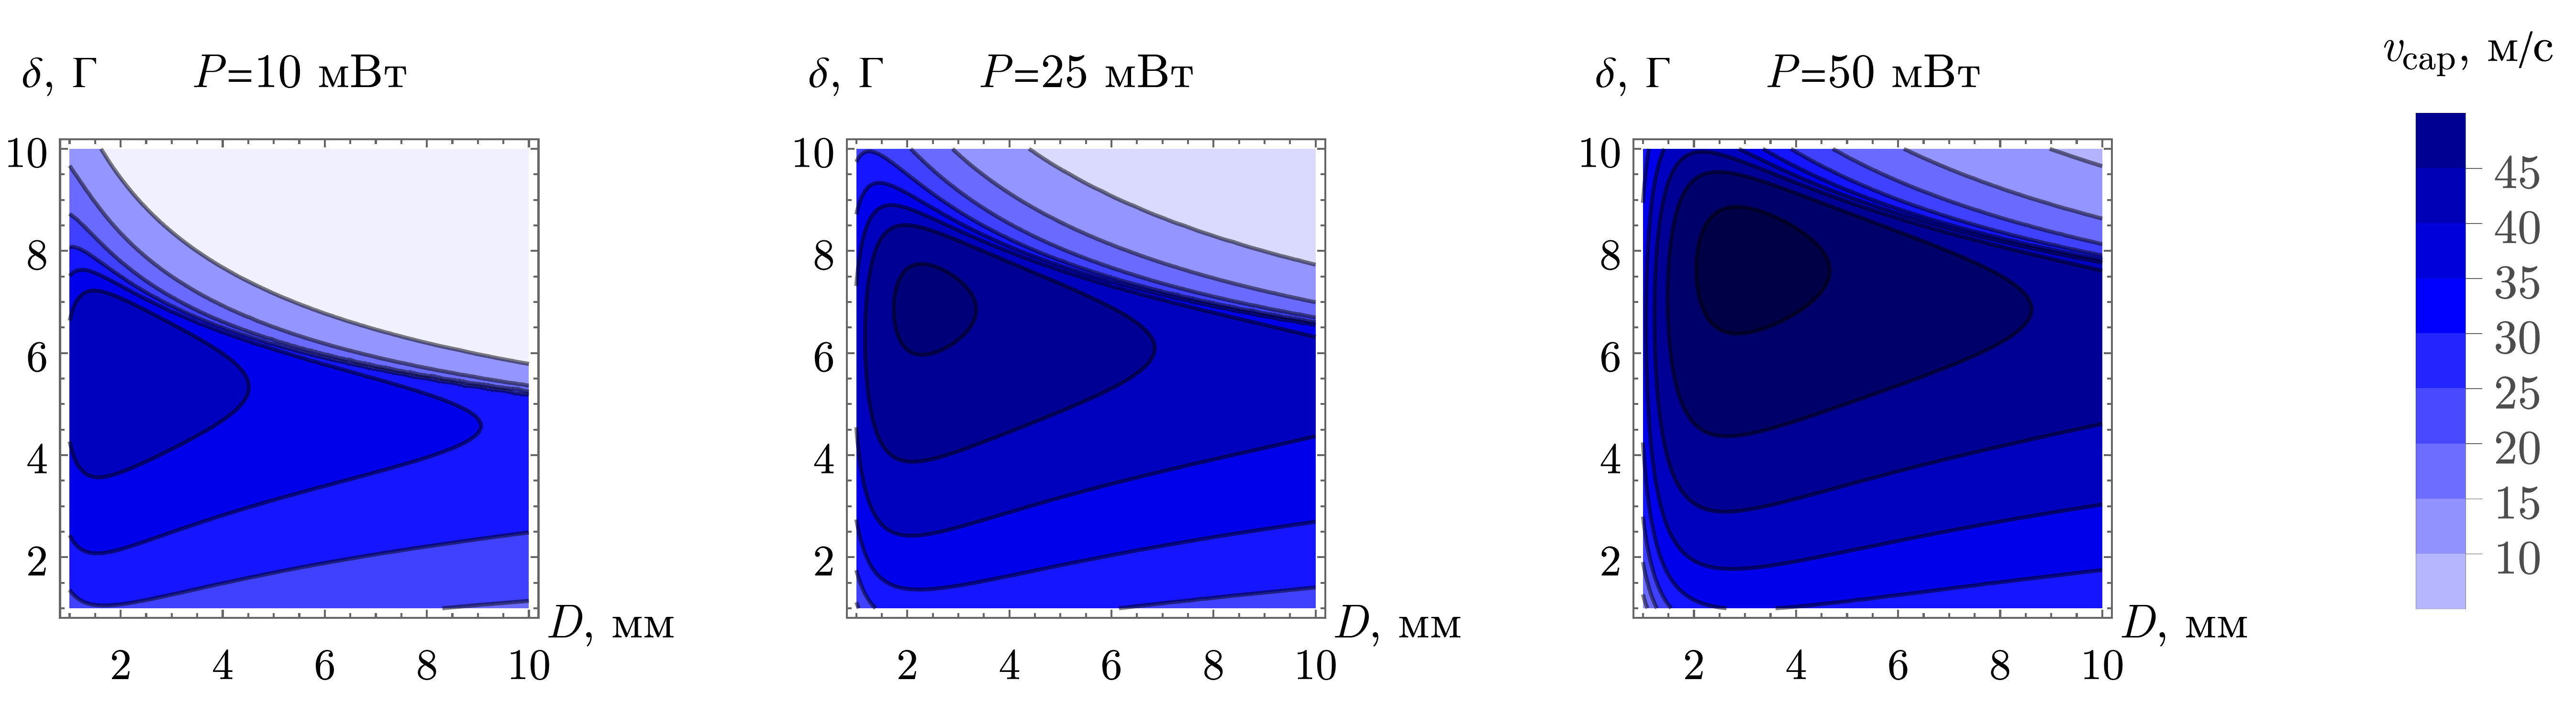
\includegraphics[width=1.0\textwidth]{figs/vcap2d_delta-Ds.png}
    \caption{Зависимость скорости захвата 2D-МОЛ для различных мощностей}
    \label{fig:vcapDs}
\end{figure}

Для наглядности представлены зависимости $\vcap(\delta, P, D=\text{5 мм})$: рис. \ref{fig:vcapflat}a, и $\vcap(\delta, P=\text{25 мВт}, D)$: рис. \ref{fig:vcapflat}b.


\begin{figure}[ht]
    \centering
    \subfigure[]{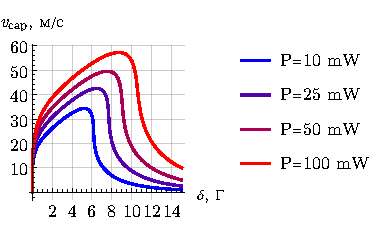
\includegraphics{figs/vcap2D_P.pdf}} %D=5мм
    \hspace{10 mm} 
    \subfigure[]{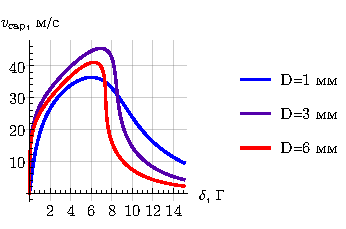
\includegraphics{figs/vcap2D_D.pdf}} %P=25мВт
    \vspace{-3mm}
    \caption{Зависимость скорости захвата от отстройки 
    % и a) мощности при $D=5$ мм; b) размеров луча при $P = 25$ мВт.
    }
    \label{fig:vcapflat}
\end{figure}


\upar{Толкающий луч}
Из геометрии системы $v_r / v_z < \theta$ \red{(описать кто есть кто)}, при этом $v_z < \vcap$, что приводит к $v_r < \theta \vcap \sim 1$ м/c. Под действием гравитации атомы могут просто не долетать до основной МОЛ, поэтому добавляется толкающий луч. 

Силу от одного толкающего луча можем найти в виде
\begin{equation}
	a(v) = F(v)/m = \frac{\hbar k}{m} \frac{\Gamma}{2} \frac{s}{1+s+\frac{(2 \pi \delta - k v)^2}{\Gamma^2/4}},
	\label{eq:force1}
\end{equation}
\red{где для простоты считали $\delta = 0$}. Также будем считать, что $\sub{v}{нач} = 0$, интересно найти зависимость $\sub{v}{кон}(s)$ при фиксированной величине длины разгона $l$:
\begin{equation}
	\int_{0}^{\sub{v}{кон}} \frac{v \d v}{a(v)} = \int_{0}^{l} \d l.
\end{equation}
Считая $s \gg \frac{\Gamma  m}{8 k^3 l \hbar } \sim 10^{-4}$, можем написать
\begin{equation}
	\sub{v}{кон}(l) = \left(\frac{\hbar \Gamma^3}{2 k m} ls\right)^{1/4}.
\end{equation}
Для $l\sim 20\,$см можем считать $\sub{v}{кон} \sim s^{1/4} \cdot 30\,\text{м/с}$.



Аналогично можем найти связь
\begin{equation}
		\int_{0}^{\sub{v}{кон}} \frac{\d v}{a(v)} = \int_{0}^{t} \d t,
		\hspace{0.5cm} \Rightarrow \hspace{0.5cm}
		\sub{v}{кон}(t) = \frac{\Gamma}{2}  \left(\frac{3 s t \hbar }{k m}\right)^{1/3}.
\end{equation}
Теперь можем записать связь например и на время
\begin{equation}
	t = \frac{2^{9/4}}{3} \left(\frac{k m}{s \Gamma^3 \hbar}\right)^{1/4} l^{3/4} = \frac{4}{3} \frac{l}{\sub{v}{кон}}.
	 % \approx 0.03 \frac{l^{3/4}}{s^{1/4}}.
\end{equation}
Тогда выражение на критическую длину:
\begin{equation}
	\sub{l}{крит} \sim 
	% \frac{3}{2^{3/2}} 
	\sqrt{\frac{\sub{h}{крит} \sub{v}{cap}^2}{g}},
\end{equation}
где $\sub{h}{крит}$ определяется геометрией вакуумной установки.




% \unewpage
\upar{Усиленные встречные пучки}
Так как основные требования к $\vcap$ возникают в торможение летящих из печки атомов, то имеет смысл перераспределить мощность в пучках 2D-МОЛ так, чтобы во встречных пучках было больше мощности. Данный приём аналогичен расположению двухмерной оптической патоки перед МОЛ, как мы уже делали в секции \red{??}. Подобные конфигурации обычно называются 2D${}^+$МОЛ.

Совмещая \eqref{eq:force1} и \eqref{eq:force2}, находим тормозящую силу ... \red{дописать!}
% \begin{equation*}
	
% \end{equation*}
% где $\alpha P$ мощности уходит на дополнительную патоку, а $(1-\alpha)P$ участвует в 

\begin{figure}[h]
    \centering
    \subfigure[]{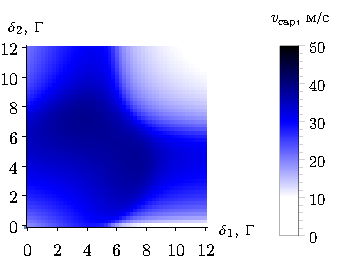
\includegraphics{figs/motplus1.pdf}}
    \hspace{20 mm} 
    \subfigure[]{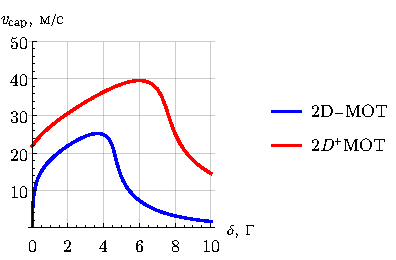
\includegraphics{figs/motplus2.pdf}} %5мм, 25 мВт
    \vspace{-3mm}
    % zeeman_sim_v2
    \caption{a) ... b) ...}
    \label{fig:motplus}
\end{figure}

